\documentclass[11pt]{article}

\usepackage{float}
\usepackage{hyperref}
\usepackage{graphicx}
% formatting
\usepackage{verbatim}
\usepackage{moreverb}
\usepackage{minted}
\usepackage{parskip}
\usepackage{amsmath}
\usepackage[listings]{tcolorbox}
\usepackage{enumerate}
\usepackage{tikz}
\usetikzlibrary{arrows,automata, positioning}
\let\verbatiminput=\verbatimtabinput
\def\verbatimtabsize{4\relax}

\newcommand{\RepoRootPath}{fpga\_labs\_fa19}

\tcbset{
texexp/.style={colframe=black, colback=lightgray!15,
         coltitle=white,
         fonttitle=\small\sffamily\bfseries, fontupper=\small, fontlower=\small},
     example/.style 2 args={texexp,
title={Question \thetcbcounter: #1},label={#2}},
}

\newtcolorbox{texexp}[1]{texexp}
\newtcolorbox[auto counter]{texexptitled}[3][]{%
example={#2}{#3},#1}

\setlength{\topmargin}{-0.5in}
\setlength{\textheight}{9in}
\setlength{\oddsidemargin}{0in}
\setlength{\evensidemargin}{0in}
\setlength{\textwidth}{6.5in}

% Useful macros

\newcommand{\note}[1]{{\bf [ NOTE: #1 ]}}
\newcommand{\fixme}[1]{{\bf [ FIXME: #1 ]}}
\newcommand{\wunits}[2]{\mbox{#1\,#2}}
\newcommand{\um}{\mbox{$\mu$m}}
\newcommand{\xum}[1]{\wunits{#1}{\um}}
\newcommand{\by}[2]{\mbox{#1$\times$#2}}
\newcommand{\byby}[3]{\mbox{#1$\times$#2$\times$#3}}


\newenvironment{tightlist}
{\begin{itemize}
 \setlength{\parsep}{0pt}
 \setlength{\itemsep}{-2pt}}
{\end{itemize}}

\newenvironment{titledtightlist}[1]
{\noindent
 ~~\textbf{#1}
 \begin{itemize}
 \setlength{\parsep}{0pt}
 \setlength{\itemsep}{-2pt}}
{\end{itemize}}

% Change spacing before and after section headers

\makeatletter
\renewcommand{\section}
{\@startsection {section}{1}{0pt}
 {-2ex}
 {1ex}
 {\bfseries\Large}}
\makeatother

\makeatletter
\renewcommand{\subsection}
{\@startsection {subsection}{1}{0pt}
 {-1ex}
 {0.5ex}
 {\bfseries\normalsize}}
\makeatother

% Reduce likelihood of a single line at the top/bottom of page
\clubpenalty=2000
\widowpenalty=2000

% Other commands and parameters
\pagestyle{myheadings}
\setlength{\parindent}{0in}
\setlength{\parskip}{10pt}

% Commands for register format figures.
\newcommand{\instbit}[1]{\mbox{\scriptsize #1}}
\newcommand{\instbitrange}[2]{\instbit{#1} \hfill \instbit{#2}}

% Break lines on texttt text on underscores
% See: https://tex.stackexchange.com/questions/315369/how-to-deal-with-bad-line-wrapping-of-texttt
\newcommand*\ttvar[1]{\texttt{\expandafter\dottvar\detokenize{#1}\relax}}
\newcommand*\dottvar[1]{\ifx\relax#1\else
  \expandafter\ifx\string_#1\string_\allowbreak\else#1\fi
  \expandafter\dottvar\fi}

\begin{document}

\def\PYZsq{\textquotesingle}
\title{\vspace{-0.4in}\Large \bf EECS 151/251A FPGA Lab 4:\\ROMs and IO Circuits\vspace{-0.1in}}

\author{Prof. Borivoje Nikolic and Prof. Sophia Shao \\
TAs: Cem Yalcin, Rebekah Zhao, Ryan Kaveh, Vighnesh Iyer \\ Department of Electrical Engineering and Computer Sciences\\
College of Engineering, University of California, Berkeley}
\date{}
\maketitle

\newcommand{\headertext}{EECS 151/251A FPGA Lab 4: ROMs and IO Circuits}
\markboth{\headertext}{\headertext}
\thispagestyle{empty}

\section{Before You Start This Lab}
Run \verb|git pull| in \texttt{\RepoRootPath}.

Review these documents that will help you better understand some concepts we will be covering.

\begin{enumerate}
  \item \href{http://inst.eecs.berkeley.edu/~eecs151/fa19/files/verilog/verilog_fsm.pdf}{verilog\_fsm.pdf} - constructing FSMs in Verilog.
  \item \href{http://www.labbookpages.co.uk/electronics/debounce.html}{Debouncer Circuit}

  Read the ``What is Switch Bounce'' section about why we need a debouncer circuit. Read the ``Digital Switch Debouncing'' section about the implementation of a debouncer circuit.
\end{enumerate}

\section{Lab Overview}
In this lab, we will
\begin{itemize}
  \item use a ROM to store a melody and play it on the FPGA using the \verb|tone_generator|
  \item build input conditioning circuits that make control signals from physical input devices, like the buttons and switches we've been using up to now, more reliable
  \item verify the conditioning circuits are working correctly using the FPGA LEDs
  \item use synchronous resets to reset our circuits to a known initial state
  \item create a basic FSM in the \verb|music_streamer| that uses the buttons to change states and alter the music playback
\end{itemize}

\section{Using an Asynchronous ROM to Build the Music Streamer}
An asynchronous memory is a memory block that isn't governed by a clock.
In this lab, we will use a Python script to generate a Verilog ROM block.

A ROM is a read-only memory.
The ROM's data can be accessed by supplying an address; after some time, the ROM will output the data stored at that address.
The number of addresses in a memory is called its \textbf{depth}, while the number of bits stored per address is called the \textbf{width} of the memory.

The synthesizer takes the Verilog you write and converts it into a low-level netlist which uses only the primitives available on the FPGA.
Our Verilog \textbf{describes} the functionality of some digital circuit and the synthesizer \textbf{infers} what primitives implement the functional description.
In this section, we will examine the Verilog that allows the synthesizer to infer a ROM.
This is a minimal example of a ROM in Verilog: (depth of 8 entries/addresses, width of 12 bits)

\begin{minted}[tabsize=2]{verilog}
module rom (input [2:0] address, output reg [11:0] data);
  always @(*) begin
    case(address)
      3'd0: data = 12'h000;
      3'd1: data = 12'hFFF;
      3'd2: data = 12'hACD;
      3'd3: data = 12'h122;
      3'd4: data = 12'h347;
      3'd5: data = 12'h93A;
      3'd6: data = 12'h0AF;
      3'd7: data = 12'hC2B;
    endcase
  end
endmodule
\end{minted}

To power our \verb|tone_generator|, we will be using a ROM that is X entries/addresses deep and 24 bits wide.
The ROM will contain notes that the \verb|tone_generator| will play.
You can choose the depth of your ROM based on how long the music is.
%the length of the sequence of tones you want to play.

We've provided you with a few scripts that can generate a ROM from either a file with it's contents or even from sheet music.
Run these commands from \verb|lab4/|.

\begin{minted}{bash}
python3 scripts/musicxml_parser.py musicxml/Twinkle_Twinkle_Little_Star.mxl music.txt
python3 scripts/rom_generator.py music.txt src/rom.v 1024 24
\end{minted}

The first script will parse a MusicXML file and turn it into a list of \verb|tone_switch_periods| for each of the notes for a piece of sheet music.
The second script will take that list and turn it into a ROM that's 1024 entries deep with a width of 24 bits.

Look at \verb|music.txt| and \verb|src/rom.v|.
The \verb|last_address| port of the ROM outputs the last address that contains a valid note.

You can download your own music in MusicXML format from here (\url{https://musescore.org/}) and run it through the same parser; it should ideally only have one part to work properly.
You can also directly edit the \verb|music.txt| file to customize the contents of the ROM as you wish.

\section{Designing the music\_streamer}
Open up the \verb|music_streamer.v| file.
You should instantiate the ROM you created earlier and add logic to address the ROM sequentially.
The \verb|music_streamer| will play each note in the ROM for a predefined amount of time by sending it to the \verb|tone_generator| via the \verb|tone| output port.
You should play each note for \textbf{1/25th of a second}.

In this section, only concern yourself with the \verb|clk| input and the \verb|tone| output; leave the other inputs unused.

Next we'll cover some testbench constructs and test the \verb|music_streamer|.

%Next, write the RTL that will increment the address supplied to the ROM every \textbf{1/25th of a second}.
%The data coming out of the ROM should be fed to the \verb|tone| output.
%The ROM's address input should go from 0 to the depth of the ROM and should then loop around back to 0. You don't have a reset signal, so define the initial state of any registers in your design for simulation purposes. Also hook up the \verb|rom_address| output to the ROM address currently being accessed.

%Now that you have implemented \verb|music_streamer|, create an instance of it in the module \verb|z1top.v|. Use the instance name \verb|streamer| to match the expected name in the \verb|.do| file. Instantiate a \verb|tone_generator| and wire \verb|SWITCHES[1]| to \verb|output_enable|, \verb|CLK_125MHZ_FPGA| to \verb|clk|, and \verb|aud_pwm| to \verb|square_wave_out|.  Assign \verb|aud_sd| to 1.  Connect the \verb|tone| output of the \verb|music_streamer| to the \verb|tone_switch_period| input of the \verb|tone_generator|. Connect the \verb|music_streamer|'s \verb|clk| input to the global clock signal. Finally, connect  its \verb|rom_address| output to the \verb|LEDS|s by routing the top 6 bits of address.

\section{Testbench Techniques} \label{sec:testbenchtechniques}
There are several testbenches included in this lab for your synchronizer, edge detector, shift register, debouncer, and music streamer that introduce you to some useful Verilog testbench constructs.
See Discussion 3 for more slides and example code.

\begin{itemize}
\item \verb|@(posedge <signal>)| and \verb|@(negedge <signal>)| - These are a different type of delay statement from what you have seen before. \verb|#10| would advance the simulation by 10 timesteps. These commands will advance the simulation until the \verb|<signal>| rises or falls.

For example:
\begin{minted}[frame=single]{verilog}
@(posedge signal);
@(posedge signal);
\end{minted}

Simulation time will advance until we have seen two rising edges of \verb|signal|.

\item \verb|repeat| - it acts like a \verb|for| loop but without an increment variable

For example:
\begin{minted}[frame=single, tabsize=4]{verilog}
repeat (2) @(negedge clk);
repeat (10) begin
  @(posedge clk);
end
\end{minted}

The simulation will advance until we have seen 2 falling clock edges and will then advance further until we have seen 10 rising clock edges.

\item \verb|$display| - acts as a print statement. Similar to languages like C, if you want to print out a wire, reg, integer, etc... value in your testbench, you will need to format the string. It works like \verb|printf()| in C.

For example:
\begin{minted}[frame=single]{verilog}
$display("Wire x in decimal is %d", x);
$display("Wire x in binary is %b", x);
\end{minted}

\item \verb|tasks| - tasks are subroutines where you can group and organize some commands rather than haphazardly putting them everywhere. They can take inputs and assign outputs.

\begin{minted}[frame=single, tabsize=4]{verilog}
task wait_for_n_clocks();
input [7:0] num_edges;
begin
  repeat (num_edges) @(posedge clk);
end
endtask
\end{minted}

\item \verb|fork/join| - Allows you to execute testbench code in parallel. You create a fork block with the keyword \verb|fork| and end the block with the keyword \verb|join|.

For example:
\begin{minted}[frame=single, tabsize=4]{verilog}
fork
  begin
    task1();
  end
  begin
    $display("Another thread");
    task2();
  end
join
\end{minted}

Multiple threads of execution are created by putting multiple begin/end blocks in the fork-join block.
In this example, thread 1 runs \verb|task1()|, while thread 2 first \verb|$display|s some text then runs \verb|task2()|.
The threads operate in parallel.

\item Hierarchical Paths - you can access signals inside an instantiated module for debugging purposes. This can be helpful in some cases where you want to look at an internal signal but don't want to create another output port just for debug.

For example:
\begin{minted}[frame=single, breaklines]{verilog}
tone_generator tone_gen ();
\$display("Signal inside my tone_generator instance, counter: %b", tone_gen.counter);
\end{minted}
\end{itemize}

\section{Simulating the music\_streamer}
To simulate your \verb|music_streamer| open up \verb|lab4/src/music_streamer_testbench.v|.
Note how the \verb|tone_generator| is wired to the \verb|music_streamer|.
This test just runs the \verb|music_streamer| for a second.

Run the test with \ttvar{make} \ttvar{sim/music_streamer_testbench.vpd} for VCS or \ttvar{make} \ttvar{sim/music_streamer_testbench.fst} for Icarus Verilog.

Inspect the waveform and verify that there are no undefined signals (red lines/X).
Run the Python script \verb|python3 scripts/audio_from_sim.py sim/output.txt| to generate a \verb|.wav| file and listen to the \verb|music_streamer|.
It should sound like the first second of the song that was loaded on the ROM.

\subsection{Verify your Code Works For Rest Notes}
In simulation, you can often catch bugs that would be difficult or impossible to catch by running your circuit on the FPGA.
You should verify that if your ROM contains an entry that is zero (i.e. generate a 0Hz wave), that the \verb|tone_generator| holds the \verb|square_wave_out| output at either 1 or 0 with no oscillation.

\begin{texexptitled}{Music Streamer Simulation}{}
  \begin{enumerate}[a)]
    \item Save a waveform screenshot demonstrating that a \verb|tone_switch_period| of 0 sent by the ROM results in no oscillation of the \verb|square_wave_out| output for checkoff.
    \item Save an audio file from the \ttvar{music_streamer} simulation for checkoff.
  \end{enumerate}
\end{texexptitled}

\subsection{FPGA Time}
Instantiate the \ttvar{music_streamer} and \ttvar{tone_generator} in \ttvar{src/z1top.v} similar to the \ttvar{music_streamer_testbench}.
Connect \verb|SWITCHES[0]| to the \verb|tone_generator|'s \verb|output_enable| and wire the \verb|volume| input to 0.
Run \verb|make impl| and \verb|make program| and hear the music played from the FPGA.

\section{Input Conditioning Circuits}
We want to use the buttons on the Pynq board to control the playback of the music by adjusting the tempo, or pausing the music and playing it in reverse.
To safely use the button signals, we have to design input conditioning circuits to handle metastability and button bounce.

\subsection{Synchronizer}
In Verilog (RTL), digital signals are either 0's or 1's.
In a digital circuit, a 0 or 1 corresponds to a low or high voltage.
If the circuit is well designed and timed (fully synchronous), we only have to worry about the low and high voltage states.

The signals coming from the push buttons and slide switches on the Pynq board don't have an associated clock (asynchronous).
When the button signals are put through a register, its hold or setup time may be violated.
This may put that register into a \textit{metastable} state (Figure \ref{fig:metastability}).

\begin{figure}
  \centerline{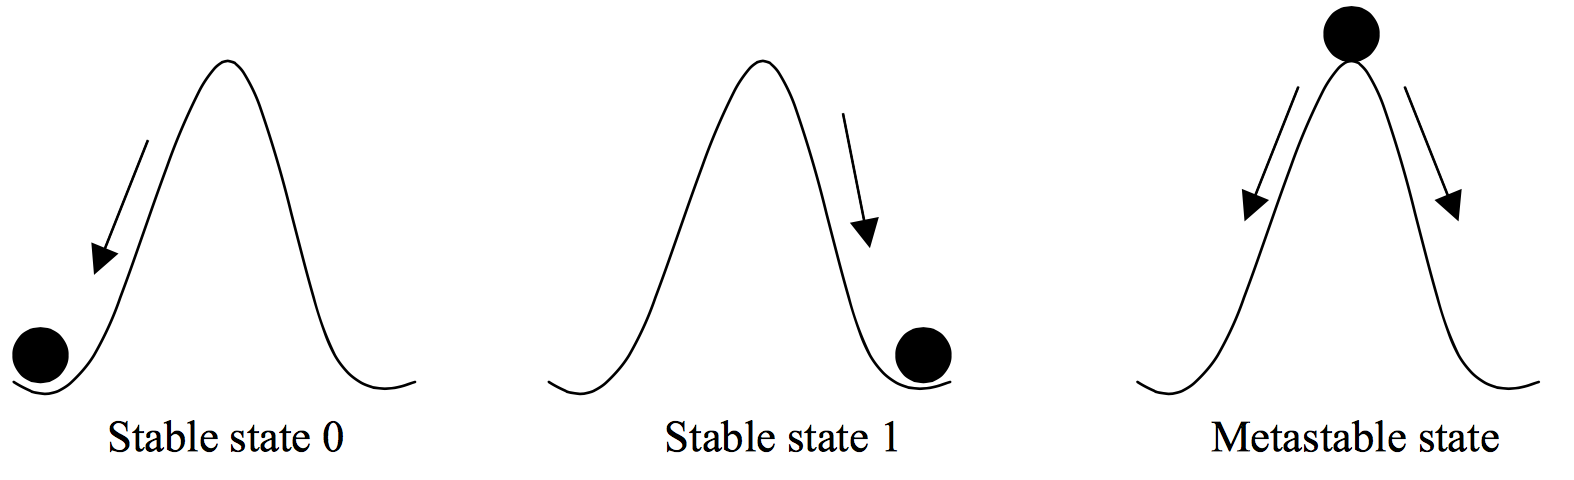
\includegraphics[height=3cm]{figs/metastability.png}}
  \caption{The `ball on a hill' metaphor for metastability. If a register's timing constraints are violated, its output voltage oscillates and after some time unpredictably settles to a stable state.}
  \label{fig:metastability}
\end{figure}

In a fully synchronous circuit, the timing tools will determine the fastest clock frequency under which the setup time constraints are all respected and the routing tools will ensure that any hold time constraints are handled.
An asynchronous signal could violate those constraints, and cause a `mid-rail' voltage from a register to propagate to other logic elements.
This can cause catastrophic timing violations that the tools never saw coming.

We will implement a synchronizer circuit that will safely bring an asynchronous signal into a synchronous circuit.
The synchronizer needs to have a very small probability of allowing metastability to propagate into our synchronous circuit.

This synchronizer circuit for this lab is relatively simple (Figure \ref{fig:synchronizer}).
For synchronizing one bit, it is a pair of flip-flops connected serially.

\begin{figure}[H]
  \vspace{0.5cm}
  \centerline{\includegraphics[width=0.4\textwidth]{figs/synchronizer.png}}
  \caption{1-bit 2 Flip-Flop Synchronizer}
  \label{fig:synchronizer}
\end{figure}

Edit \verb|src/synchronizer.v| to implement the two flip-flop synchronizer.
This module is parameterized by a \verb|width| parameter which controls the number of one-bit signals to synchronize.

\subsubsection{Synchronizer Simulation}
A test is provided in \ttvar{sim/sync_testbench.v}.
Run it as usual \ttvar{make sim/sync_testbench.vpd}.
For details on the constructs/techniques/syntax used in this testbench, refer to Section \ref{sec:testbenchtechniques}.

\subsection{Debouncer}
\begin{figure}[H]
  \centerline{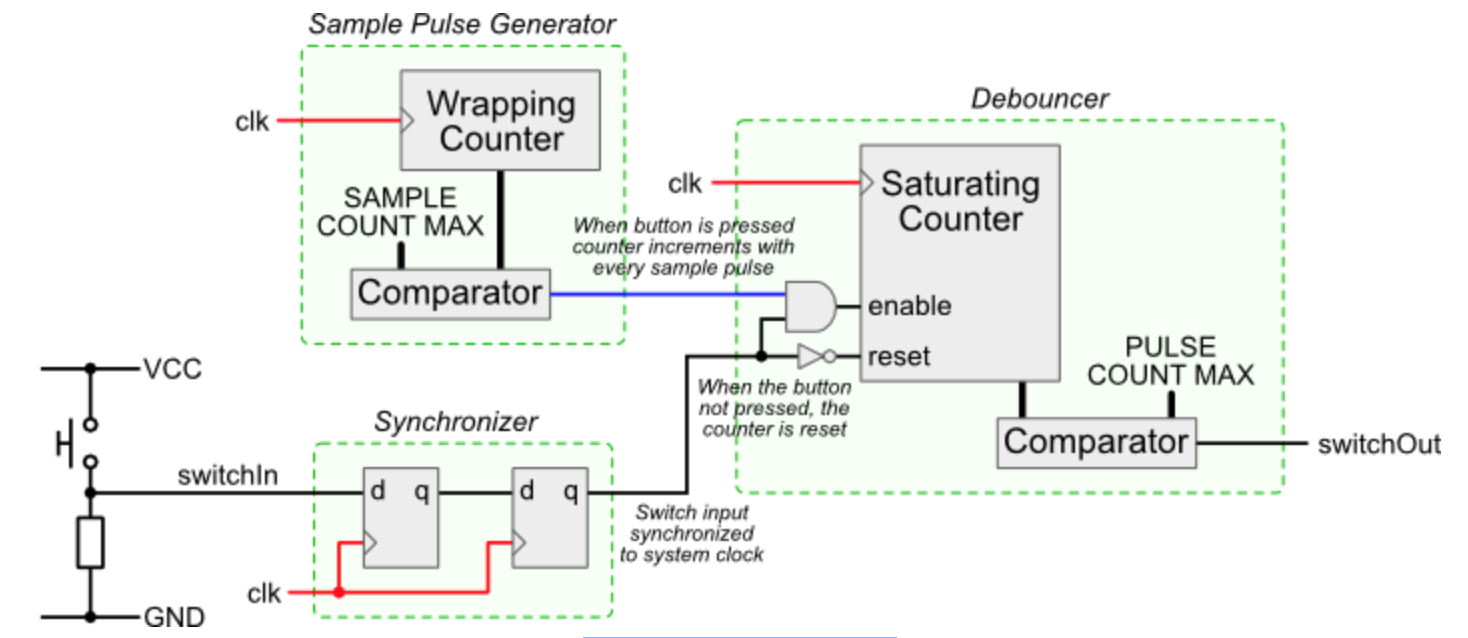
\includegraphics[height=5cm]{figs/debouncer.png}}
\end{figure}

Recall this graphic from the prelab debouncer reading.

The debouncer circuit takes a button's glitchy digital signal and outputs a clean signal indicating a single button press.
The reason we need a circuit for this can be seen in the figure below.

\begin{figure}[H]
  \centerline{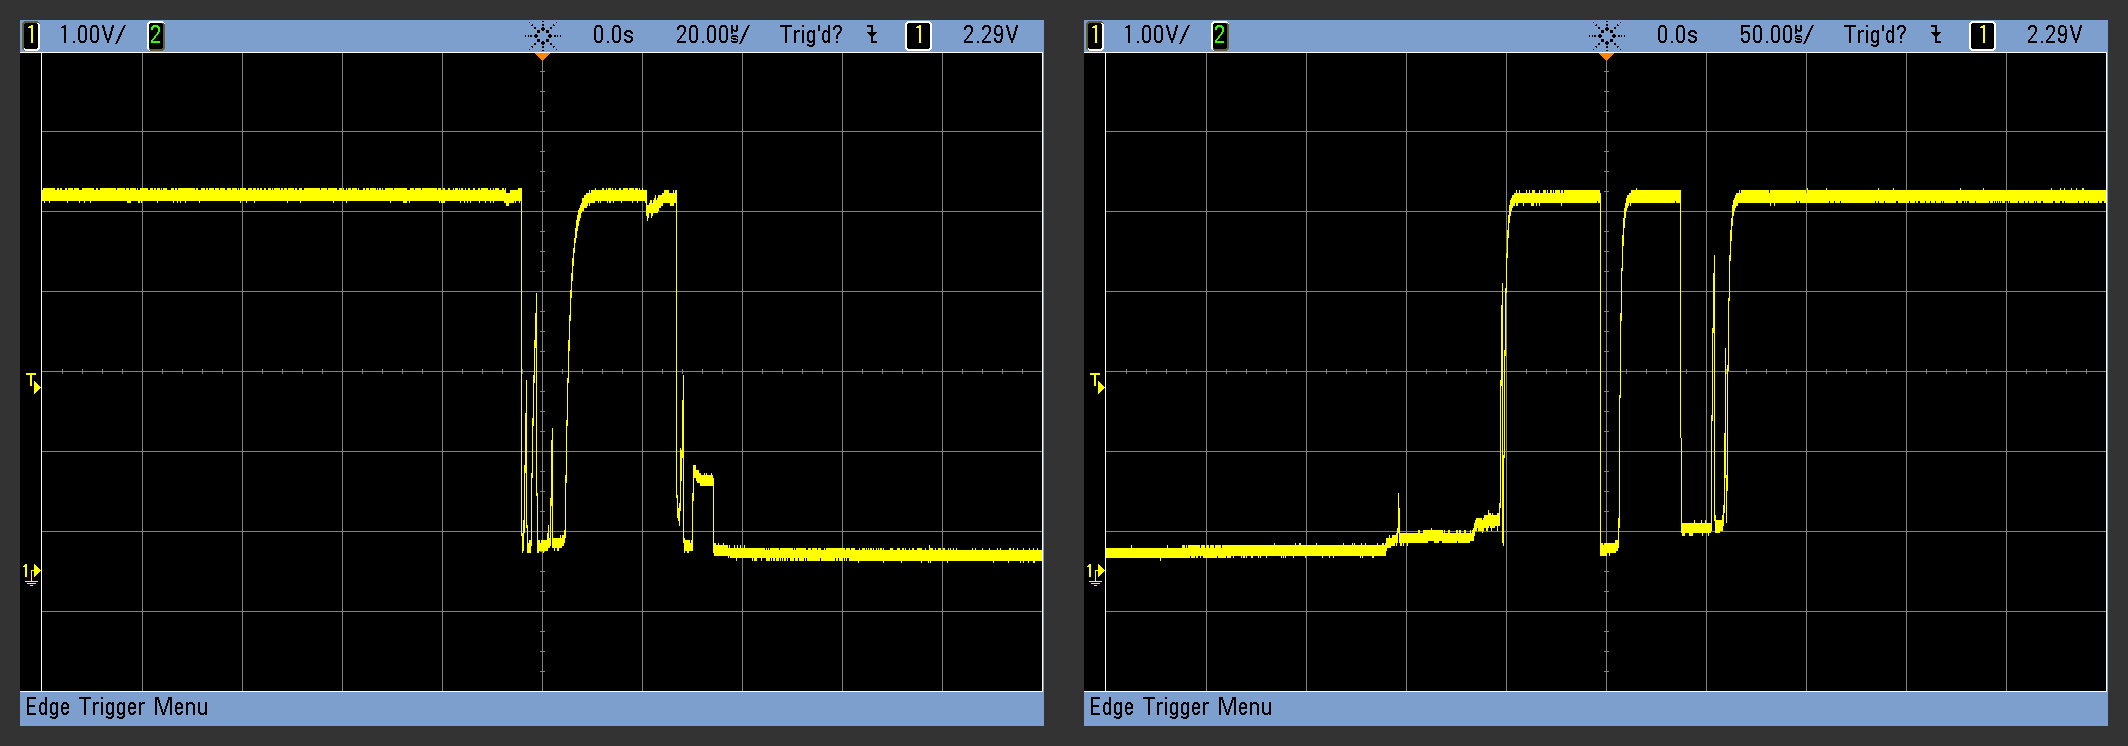
\includegraphics[width=0.5\textwidth]{figs/bouncing.png}}
\end{figure}

When we press or depress a button, the signal doesn't behave like a perfect step function.
Instead the button signal is glitchy due to mechanical ``bounce''.
If we naively used the button signal directly there would be many spurious ``button presses".

Look at \verb|src/debouncer.v|.
This is a parameterized debouncer which can debounce \verb|width| signals at a time.
The other parameters reference the constants used in the circuit from the prelab reading.

The debouncer consists of:
\begin{enumerate}
  \item \textbf{Sample Pulse Generator} - Tells our saturating counter when to sample the input signal. It should output a 1, every \verb|sample_count_max| clock cycles. By default \verb|sample_count_max| is set to 25000.
  \item \textbf{Saturating Counter} - This is a counter that counts up to \verb|pulse_count_max|.
    If the sample pulse is high at a clock edge, increment the counter if the input signal is also high, else reset the counter to 0.
    Once the saturating counter reaches \verb|pulse_count_max|, it should hold that value indefinitely until the sampled input signal becomes 0.
    The \verb|debounced_signal| of your debouncer should be an equality check between the saturating counter and \verb|pulse_count_max|.
\end{enumerate}

You can use the same sample pulse generator for all input signals into your \verb|debouncer|, but you should have a separate saturating counter per input signal.
You will likely need to use a 2D reg in Verilog to create the saturating counters. You may need to use generate-for.

Here is an \textit{example} of creating a 2D array:

\begin{minted}[tabsize=4]{verilog}
reg [7:0] arr [3:0]; // 4 X 8 bit array
arr[0]; // First byte from arr (8 bits)
arr[1][2]; // Third bit of 2nd byte from arr (1 bit)
\end{minted}

And here is an \textit{example} of using a generate-for loop:
\begin{minted}[tabsize=4]{verilog}
genvar i;
generate
  for (i = 0; i < width; i = i + 1) begin:LOOP_NAME
    always @ (posedge clk) begin
      // Insert synchronous Verilog here
    end
  end
endgenerate
\end{minted}
Implement the debouncer.

\subsubsection{Debouncer Simulation}
A testbench has been provided in \verb|sim/debouncer_testbench.v|. Make sure you understand what the testbench is doing. Run it as usual.

The debouncer testbench has 2 tests:
\begin{enumerate}
  \item Verifies that if a glitchy signal initially bounces and then stays high for \textbf{less} than the saturation time, that the debouncer output never goes high.
  \item Verifies that if a glitchy signal initially bounces and then stays high for \textbf{more} than the saturation time, that the debouncer goes high and stays high until the glitchy signal goes low.
\end{enumerate}

If you are seeing issues where certain registers are red lines (X's), make sure you give them an initial state. For a 2D reg initialization, use the following initialization code in \verb|debouncer.v|:
\begin{minted}[tabsize=4]{Verilog}
integer k;
initial begin
  for (k = 0; k < width; k = k + 1) begin
    saturating_counter[k] = 0;
  end
end
\end{minted}

\subsection{Edge Detector}
The debouncer will act to \emph{smooth-out} the button press signal.
It is then followed up with an edge detector that can take the low-to-high transition of the debouncer output and use it to generate a 1 clock cycle wide pulse that the rest of our digital design can use.

Create a variable-width edge detector in \verb|src/edge_detector.v|.

\subsubsection{Edge Detector Simulation}
A testbench is provided in \verb|edge_detector_testbench.v|. Run as usual.

The edge detector testbench tests 2 scenarios, when the \verb|signal_in| is a pulse 10 clock cycles wide and a pulse 1 clock cycle wide and verifies that the \verb|edge_detect_pulse| output goes high twice, both times with a width of 1 clock cycle.

\subsection{Input Conditioning Circuits on the FPGA}
Look at \verb|src/button_parser.v| which combines the synchronizer, debouncer, and edge detector in a chain.
A test of the \ttvar{button_parser} is in \verb|src/z1top.v| which contains a 4-bit \verb|count| register which is incremented/decremented by pressing buttons.
The LEDs show the current value of \verb|count|.

Run \verb|make lint| and \verb|make program| and try the circuit on the FPGA.
Make sure to check synthesis warnings in \verb|build/synth/synth.log|. Fix any that are unexpected.
Check that each button performs the right action on the FPGA.

\section{Synchronous Resets In Design and Simulation}
Now that we have a debouncer that can give us a pulse for a press of a button, we have a way of explicitly resetting our circuits!
You will recall that in the previous lab, we set the initial value of registers as below so that our simulation would have defined signals.

\begin{minted}[tabsize=4]{verilog}
reg [23:0] counter = 0;
\end{minted}
or
\begin{minted}[tabsize=4]{verilog}
initial counter = 0;
\end{minted}

Tying one of the push buttons to a reset signal, we can now do this instead.

\begin{minted}[tabsize=4]{verilog}
always @ (posedge clk) begin
  if (rst) begin
    counter <= 24'd0;
  end
  else begin
    counter <= counter + 24'd1;
  end
end
\end{minted}

Unlike what we did before, this Verilog is synthesizable for all deployment targets, FPGAs, ASICs, and CPLDs.
Modify the \verb|tone_generator| and \verb|music_streamer| to use the provided \verb|rst| signal instead of initial assignemnts.

Try rerunning the \verb|music_streamer_testbench|, which pulses the \verb|rst| signal, and verify using the waveform that there are no Xs.

Finally connect \verb|buttons_pressed[0]| to the \verb|music_streamer| and \verb|tone_generator| \verb|rst| input in \verb|z1top.v|.
Program the FPGA and verify the reset functionality.

\section{Music Streamer Tempo Control}
Let's use the new user inputs we now have access to.
The \verb|music_streamer| plays each tone in the ROM for 1/25th of a second.

Use the \verb|tempo_up| and \verb|tempo_down| inputs to the \ttvar{music_streamer} to decrease and increase respectively the time each tone in the ROM is played.

%Extend the functionality of the \verb|music_streamer| so that one input increases the tempo, one input decreases it, and one resets it to a default value. If you have the hex keypad working, you can map any of the keys to these functions, but make a note of it. If not, use the push-buttons left on the Pynq-Z1 (remembering that BTN3 is now reserved as a global reset signal).

You can implement this by using a register to hold the number of clock cycles per note.
Instead of this number being hardcoded in Verilog to represent $\frac{1}{25}$th of a second, you can change it at runtime.
You can add or subtract a fixed number from this register, which should alter the time each tone is played.
You get to choose this number.

Next in \verb|z1top.v|, delete the \ttvar{button_parser} test circuit and connect the \verb|music_streamer| as such:
\begin{itemize}
  \item \verb|tempo_up = SWITCHES[1] & buttons_pressed[1]|
  \item \verb|tempo_down = !SWITCHES[1] & buttons_pressed[1]|
\end{itemize}

Try it out on the FPGA and verify that you have control of your \verb|music_streamer|'s tempo using the buttons.

\section{Checkoff}
\begin{enumerate}
  \item Show the RTL for the input conditioning circuits and music streamer
  \item Show a waveform demonstrating no oscillation if the \verb|tone_switch_period| is 0
  \item Play an audio file generated from a simulation
  \item Demonstrate the music streamer on the FPGA (tempo control, reset)
  \item Explain how the \verb|debouncer_testbench|, \verb|edge_detector_testbench|, and \verb|sync_testbench| work. Why do we use fork-join?
\end{enumerate}

\subsection{Lab Report}
No lab report for this lab!

\section*{Ackowlegement}
This lab is the result of the work of many EECS151/251 GSIs over the years including:
\begin{itemize}
\item Sp12: James Parker, Daiwei Li, Shaoyi Cheng
\item Sp13: Shaoyi Cheng, Vincent Lee
\item Fa14: Simon Scott, Ian Juch
\item Fa15: James Martin
\item Fa16: Vighnesh Iyer
\item Fa17: George Alexandrov, Vighnesh Iyer, Nathan Narevsky
\item Sp18: Arya Reais-Parsi, Taehwan Kim
\item Fa18: Ali Moin, George Alexandrov, Andy Zhou
\end{itemize}

\end{document}
